\documentclass{article}
\usepackage[ngerman]{babel}
\usepackage[utf8]{inputenc}
\usepackage[T1]{fontenc}
\usepackage{graphicx}
\usepackage{color}
\usepackage{xcolor}
\usepackage{listings}
\usepackage{comment}
\usepackage{tikz}
\usepackage{enumitem}

\newcommand{\circled}[1]{
    \setbox0=\hbox{#1}%
    \dimen0\wd0%
    \divide\dimen0 by 2%
    \begin{tikzpicture}[baseline=(a.base)]%
        \useasboundingbox (-\the\dimen0,0pt) rectangle (\the\dimen0,1pt);
        \node[circle,draw,outer sep=0.6pt,inner sep=0.3ex] (a) {#1};
    \end{tikzpicture}
}

\newcommand{\circledsmall}[1]{
    \setbox0=\hbox{#1}%
    \dimen0\wd0%
    \divide\dimen0 by 2%
    \begin{tikzpicture}[baseline=(a.base)]%
        \useasboundingbox (-\the\dimen0,0pt) rectangle (\the\dimen0,1pt);
        \node[circle,draw,outer sep=0pt,inner sep=0.3ex] (a) {#1};
    \end{tikzpicture}
}

\renewcommand{\lstlistingname}{Auflistung}

\colorlet{punct}{red!60!black}
\definecolor{background}{HTML}{FFFFFF}
\definecolor{delim}{RGB}{20,105,176}
\colorlet{numb}{magenta!60!black}

\lstdefinelanguage{json}{
    basicstyle=\normalfont\ttfamily,
    numbers=left,
    numberstyle=\scriptsize,
    stepnumber=1,
    numbersep=8pt,
    showstringspaces=false,
    breaklines=true,
    frame=lines,
    backgroundcolor=\color{background},
    literate=
     *{0}{{{\color{numb}0}}}{1}
      {1}{{{\color{numb}1}}}{1}
      {2}{{{\color{numb}2}}}{1}
      {3}{{{\color{numb}3}}}{1}
      {4}{{{\color{numb}4}}}{1}
      {5}{{{\color{numb}5}}}{1}
      {6}{{{\color{numb}6}}}{1}
      {7}{{{\color{numb}7}}}{1}
      {8}{{{\color{numb}8}}}{1}
      {9}{{{\color{numb}9}}}{1}
      {:}{{{\color{punct}{:}}}}{1}
      {,}{{{\color{punct}{,}}}}{1}
      {\{}{{{\color{delim}{\{}}}}{1}
      {\}}{{{\color{delim}{\}}}}}{1}
      {[}{{{\color{delim}{[}}}}{1}
      {]}{{{\color{delim}{]}}}}{1},
}

\newcommand*{\signature}[2]{%
    \par\noindent\makebox[2.0in]{\hrulefill} \hfill\makebox[2.0in]{\hrulefill}%
    \par\noindent\makebox[2.0in][l]{Unterschrift #1}      \hfill\makebox[2.0in][l]{Unterschrift #2}%
}%

\newcommand{\blankpage}{
\newpage
\thispagestyle{empty}
\mbox{}
\newpage
}

\setlength{\parindent}{0pt}

\begin{document}
\shorthandoff{"}

\begin{titlepage}
  \topmargin0mm
  \setlength{\parindent}{0em}

\begin{minipage}{\textwidth}
    \centering
    \vspace{0.8cm}
    \begin{large}Hochschule RheinMain\\
    Fachbereich Design Informatik Medien\\
    Studiengang Angewandte Informatik\end{large}
\end{minipage}

\begin{minipage}{\textwidth}
    \centering	
    \vspace{0.8cm}
   \begin{large} 
Praktikumsbericht
	\end{large}    
    \vspace{4cm}
    \renewcommand{\baselinestretch}{1}
    \small\normalsize
\end{minipage}

  \vspace{6.5cm}
  vorgelegt von Kevin Sapper\\
  \\
  am 26. Juli 2014\\
  \\
  \\
  \\
	Betreuer HS RM: 	Prof. Dr. Kröger\\
  \\
	Betreuer in Fa.: 	Matthias Wolf
  \cleardoublepage
\end{titlepage}

\blankpage

\thispagestyle{empty}
\vspace*{\fill}
Hiermit wird bestätigt, dass der Bericht selbständig vom Studierenden erstellt wurde und in seinem Inhalt der Wahrheit entspricht.
\\
\\
\\
\signature{Betreuer in Fa.}{Studierender}
\clearpage

\pagenumbering{Roman}
\setcounter{tocdepth}{2}
\tableofcontents
\clearpage

\clearpage	
\pagenumbering{arabic}
\pagestyle{plain}

\section{Einleitung}

Als Teil der praktischen Hochschulausbildung dient im 6ten Semester das Praxisprojekt. In diesem Rahmen wurden 420 Stunden praktischer Tätigkeit bei der Eckelmann AG, in Wiesbaden-Erbenheim, absolviert. Die Eckelmann AG ist ein mittelständisches Unternehmen mit ca. 350 Mitarbeitern und einer Firmengeschichte von über 35 Jahren. Sie wurde im Jahr 1977 von Dr. Gerd Eckelmann als  Dr.-Ing. Eckelmann GmbH gegründet. Im Jahre 2001 findet die Umwandlung zur Eckelmann AG statt. Zur Eckelmann AG gehören mittlerweile 5 Tochtergesellschaften, davon drei in Deutschland, eine in China und eine in Tschechien. Seit 1986 gibt es den Standort in Erbenheim. Dieser wurde 2013 durch ein weiteres Gebäude um 1600 Quadratmeter erweitert. Spezialisiert ist das Unternehmen in der elektrischen Automation von Maschinen und Anlagen. Die Leistungen gliedern sich dabei in die Bereiche Elektronische Entwicklung und Fertigung, Software-Entwicklung, Elektroanlagen und Schaltschrankbau sowie Vorgehensmodelle für die Entwicklung. Diese Leistungen werden in vielen verschiedenen Branchen, wie z.B. Maschinenbau, Chemie \& Pharma, Schiffbau oder Industriekälte \& Gewerbekälte, erbracht.

Das Praktikum hat in der Abteilung Kälte- und Gebäudeleittechnik im Team Datentechnik stattgefunden. Im Bereich Kältetechnik wird Regelungstechnik zur Vernetzung und Überwachung von Kälteanlagen entwickelt. Hierzu gehören die Produkte aus der E*LDS Reihe. Diese beinhalten Verbundsteuerungen zur Kälteerzeugung, Kühlstellenregler zur temperaturgenauen Reglung aller Arten von Kühlmöbeln und Kühlräumen, Funk-Temperatursensoren und der Marktrechner als zentrale Intelligenz einer Kälteanlage. Der Betrieb einer Kälteanlage hat zahlreiche Seiteneffekte, welche Synergiepotenzial in der Gebäudeleittechnik hat. Einer der Synergieeffekte ist die Nutzung der Abwärme, welche teilweise oder komplett konventionelle Heizungen und Warmwasseraufbereitung ersetzen kann.

Das Team Datentechnik besteht aus 9 Entwicklern, welche Software für den Marktrechner entwickeln. Weiter gibt es einige Erweiterungen wie z. B. ein Gateway zum Local Area Network (LAN).
\pagebreak


\section{Projektbericht}

Für die Verwaltung und Überwachung einer Kälteanlage ist es notwendig, Werte auszulesen und auszuwerten. Anhand der ausgewerteten Daten können dann, zur Fehlerbehandlung oder Effizienzsteigerung, Änderungen am System vorgenommen werden. Viele der Anlagen werden von Fernwarten überwacht, da sich der permanente Einsatz eines Mitarbeiters vor Ort nicht rentiert. Somit müssen die auszulesenden und auszuwertenden Werte von der Kälteanlage zu einer Fernwarte transferiert werden. Die Kommunikationswege über interne VPNs oder extern durch das Internet, werden meist durch restriktive Firewalls unterbunden. Die Anpassung der Firewallregeln ist bei der Verwaltung vieler Kälteanlagen in einer Fernwarte sehr umständlich und fehleranfällig. Zudem haben vor allem große Konzerne Richtlinien, die Anpassungen an der Firewall nicht zulassen. Einen Ausweg aus dieser Situation bietet die Kommunikation über HTTP und HTTPS. Diese wird von den meisten Firewalls erlaubt. Webservice Protokolle, welche HTTP zur Kommunikation nutzen, sind deshalb bei Entwicklern ein einfaches und beliebtes Mittel zur Lösung solcher Szenarien. Aus diesem Grund sind Webservices in heutigen Systemlandschaften weit verbreitet und daher leicht in beliebigen Programmiersprachen zu implementieren.

Im Rahmen dieses Projektes soll eine Gateway entstehen, das zur Überwachung einer Kälteanlage Webservices einsetzt.

\subsection{Problemfeld}

Es existiert bereits eine Webservice-Schnittstelle, welche einfache XML-RPCs benutzt. Diese Schnittstelle weist, durch Anforderungen unterschiedlicher Kunden, allerdings keine einheitliche Struktur auf. Der Aufbau eingehender und ausgehender XML-Dokumente ist je nach Funktion unterschiedlich. Zudem muss jede Änderung zunächst auf die Hardware aufgespielt werden. Da der Betrieb einer Kälteanlage zu Testzwecken nicht wirtschaftlich ist, müssen neue Schnittstellen bei ausgewählten Kunden getestet werden. Hierzu muss vor Ort zunächst die neue Software aufgespielt. Je nach Verfügbarkeit eines Mitarbeiters, kann das einige Tage in Anspruch nehmen. Aus diesem Grund kann sich ein Testzyklus extrem in die Länge ziehen. Weiterhin bietet die jetzige Schnittstelle keine ausreichende Möglichkeit der Autorisierung von Benutzern und Verschlüsselung von Daten.

\subsection{Aufgabenstellung}

Das Projekt stellt folgende Anforderungen, welche im Rahmen der Implementierung eingehalten werden sollen. Zunächst wird die Anforderung gestellt möglichst keine Firewalleinstellungen zur Inbetriebnahme verändern zu müssen. Die Protokolle HTTP und HTTPS sind für die meisten Firewalls am unproblematischsten. Des Weiteren soll das Gateway zustandsfrei arbeiten, um den serverseitigen Aufwand zu reduzieren. Es muss in der Lage sein lokal mit eingeschränkten Hardwareressourcen zu laufen. Der Testzyklus soll reduziert werden, indem die Software von extern gegen die Hardware funktioniert, ohne diese updaten zu müssen. Als Anforderung gegenüber dem Client muss gewährleistet werden, dass dieser die Möglichkeit hat die Repräsentation der Antwort zu bestimmen. Für die Programmierung wird C++ und das Qt-Framework empfohlen, da diese bereits in die existierende Toolchain eingebunden sind.

\subsection{Grundlagen}

Bevor weitere Details über das Projekt erklärt werden können, müssen die folgenden Grundlagen zum Verständnis geschaffen werden. Exakte Angaben zum Aufbau von Strukturen und Protokollen sind aufgrund der datenschutzrechtlichen Bestimmungen nicht möglich.

\subsubsection{REST}

REST ist ein Konzept zur Entwicklung von Services. Ihm liegen die folgenden fünf Kernprinzipien zugrunde.

\paragraph{Ressourcen mit eindeutiger Identifikation}
durch Verwendung von Uniform Resource Identifiers (URI). Diese Technik ist dank des Web sehr erprobt und für jeden leicht verständlich. URIs ermöglichen die Identifikation aller wesentlichen Instanzen einer Anwendung, egal ob es individuelle Einträge oder Mengen sind.

\paragraph{Verknüpfungen/Hypermedia}

sind bekannt als Links. Diese werden heutzutage überall im Web genutzt. Durch sie ist es möglich, Ressourcen miteinander zu verknüpfen, um den Applikationsfluss darüber zu steuern.

\paragraph{Standardmethoden}

hier im Bezug auf das Standardanwendungsprotokoll HTTP. Dieses muss von allen Teilnehmern einer REST-Schnittstelle verstanden werden.

\paragraph{Unterschiedliche Repräsentation}

von Ressourcen für unterschiedliche Anforderungen. Ein Client kann beispielsweise Daten im XML-Format verarbeiten, ein anderer allerdings nur im JSON-Format. Die Bereitstellung hierfür muss vom Service geleistet werden.

\paragraph{Statuslose Kommunikation}

REST schreibt vor, dass der Status entweder von Client gehalten oder vom Server in einen Ressourcenstatus umgewandelt werden muss.

\subsubsection{Qt}

Qt[kju:t] ist ein Cross-Plattform Framework für C++ Entwickler. Die neuste Version läuft unter Linux, Android, Mac, iOS und Windows.
\footnote{Quelle: http://qt-project.org}

\subsubsection{ZeroMQ}

ZeroMQ ist eine Netzwerk-Bibliothek, welche sich wie ein Concurrency Framework verhält. Es stellt dem Benutzer Sockets zur Verfügung, um atomare Nachrichten, über in-process (inproc), inter-process (ipc), TCP und multicast zu senden. Sockets können von verschiedenen Typen sein, die einen erprobten Mechanismus der Messaging-Technik zu Grunde liegen. Beispiele sind Publisher- und Subscriber-Sockets oder Request- und Response-Sockets. ZeroMQ erlaubt es äußerst effizient, asynchrone, skalierbare Anwendungen zu schreiben.
\footnote{Quelle: http://zguide.zeromq.org/page:all}

\subsubsection{Telegramme}

Telegramme sind Nachrichten, welche benutzt werden, um Daten über den CAN-Bus zu versenden. Ein CAN-Bus-Telegramm kann an einen einzelnen oder an alle Teilnehmer am CAN-Bus gesendet werden. Beim Versenden größerer Datenmengen kann man auf CAN-Bus-Blocknachrichten zurückgreifen. Sollte eine Blocknachricht nicht ausreichen, können beliebig viele zusammengehörige Blocknachrichten gesendet werden. Diese werden vom Empfänger als eine Nachricht interpretiert. Eine Blocknachricht bzw. eine Sequenz von Blocknachrichten wird im Gegensatz zu CAN-Bus-Telegrammen quittiert. Über die Quittung kann der Sender z. B. erfahren, ob die von ihm gesendeten Daten akzeptiert worden und plausibel sind. Das Quittieren sorgt allerdings dafür, dass CAN-Bus-Blocknachrichten nur an einen einzelnen Teilnehmer gesendet werden können. 

\subsubsection{Lan-Gateway}

Das LAN-Gateway ist  eine Software-Komponente des Marktrechners. Es übersetzt Telegramme zwischen CAN und TCP. Die Anzahl der zulässigen TCP-Verbindungen ist, durch die Software, auf 3 beschränkt. Für einen TCP-Client sind Sequenzen aus von Blocknachricht transparent, denn diese werden vom LAN-Gateway zusammengefasst und in einer Nachricht versendet.

\subsubsection{Datenpunkt}

Teilnehmer im E*LDS System können je nach Funktion eine Menge an Daten liefern. Um einen einzelnen Datenstrom zu benennen, werden Datenpunkte beschrieben, die einen Datenstrom auf einer Komponente eindeutig identifizieren.

\subsection{Konzept}

Der Idee des zu entwickelten Systems wurde in einem Grobkonzept beschrieben. Die Software wurde iterativ entwickelt, ein Feinkonzept mit den neuen Anforderungen wurde deshalb für jede Iteration entwickelt. 

\subsubsection{Grobkonzept}

Als Projektanforderung heißt es "Vermeidung von Firewalländerungen" und "zustandsfrei" zu arbeiten. Mit dem REST-Konzept wird genau dies bedient. Es baut auf dem HTTP-Protokoll auf und überlässt die Zustandsverwaltung dem Client. Die Software, im weiteren Verlauf RestGateway genannt, wird Anfragen bestehend aus einer URI, welche auf eine Ressource im E*LDS System verweist, bearbeiten. Anfragen müssen in ein Telegramm, das das E*LDS System versteht, umgewandelt werden. Dieses wird über TCP an das Gateway des Marktrechners gesendet. Hierbei ist egal, ob die TCP-Verbindung lokal über Loopback oder extern über LAN aufgebaut wird. Dadurch wird die Anforderung erfüllt einerseits lokal, andererseits extern zu funktionieren. Das Gateway am Marktrechner leitet die Anfrage an seinen eigentlichen Empfänger am CAN-Bus weiter. Falls das gesendete Telegramm eine Antwort zur Folge hat, wird diese vom Marktrechner an das RestGateway zurückgesendet. Das RestGateway muss die Antwort interpretieren. Die Anforderung den Client die Repräsentation des Rückgabedokuments bestimmen zu lassen wird durch eine Auswahl an gültigen Formaten umgesetzt. Wählbare gültige Formate sind XML- oder JSON-Dokumente. In Abbildung \ref{fig:architektur_ueberblick} sind die hier beschrieben Komponenten mit ihren Schnittstellen visualisiert.

\begin{figure}[h]
\centering
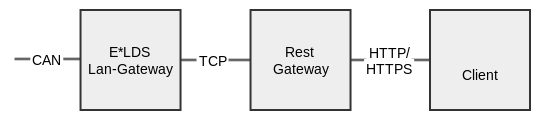
\includegraphics[scale=0.5]{Grobkonzept.png}
\caption{Komponenten und Schnittstellen der groben Architektur}
\label{fig:architektur_ueberblick}
\end{figure}

\subsection{Erste Iteration}
\label{sec:it_1}

\subsubsection{Feinkonzept}

Das RestGateway soll Informationen einer Kälteanlage liefern. Gemäß dem REST Grundprinzips "Ressourcen mit eindeutiger Identifikation" wurden in der ersten Iteration dafür relevante Instanzen des E*LDS System gesucht und mit eindeutigen URIs versehen. Insgesamt sind 28 Ressourcen mit URIs versehen worden. Der Fokus in der ersten Iteration lag dabei auf fünf Ressourcen dieser Menge. Der Aufbau einer URI wird in Abbildung ~\ref{fig:resturi} dargestellt. Auf IP und Port folgt das Schlüsselwort "REST", eine Versionsnummer und anschließend der Ressourcen identifizierende Teil. Über Parameter kann die Anfrage noch weiter spezifiziert werden.

\begin{figure}[h]
\begin{quote}
http://IP:PORT/REST/VERSION/RESSOURCE?PARAMETER
\end{quote}
\caption{Aufbau REST-URI}
\label{fig:resturi}
\end{figure}

Abbildung \ref{fig:resturi_id} zeigt eine Beispiel-URI zum Erfragen bestimmter Daten der Archivierung eines bestimmten Zählers. Der Ressourcenteil ist hier weiter unterteilt. Durch das Einsetzen einer ID wird eine konkrete Ressource benannt. Im Parameterteil gibt es allgemeine und ressourcenspezifische Parameter. Allgemeine sind "format" und "ip". Mit "format" wird der Typ des gewünschten Rückgabedokuments angegeben. Dieser ist Pflicht für jede Anfrage. Fehlt er, soll als Antwort der HTTP Statuscode 400 (Bad Request) gesendet. Über "ip" wird der Ziel-Marktrechner ausgewählt, an welchen die Anfrage gerichtet wird. Ein ressourcenspezifischer Parameter ist die Datenpunkt-ID "dpid". Viele Ressourcen bieten eine Menge an verschiedenen Datenpunkten an. Mit "dpid" wird bestimmt, von welchem Datenpunkt einer Komponente Daten abfragt werden. 

\begin{figure}[h]
\begin{quote}
/REST/1.0/zaehler/archivierung/32?format=xml\&ip=10.0.0.1\&dpid=3
\end{quote}
\caption{gekürzte REST-URI mit benannter Ressource}
\label{fig:resturi_id}
\end{figure} 

Weitere ressourcenspezifische Parameter sind "from" und "to". Über sie wird eine Datenmenge auf einen bestimmten Zeitraum eingeschränkt.

Damit die durch URIs ausgelösten Anfragen bearbeitet werden können bedarf es eines Webservers. Dieser wird durch das C++ Framework CPPCMS geliefert. Neben einem Webserver stellt dieses diverse Methoden und Funktionen, zum Auslesen der Anfrage und zum Bauen der Antwort, zur Verfügung. Der Kern von CPPCMS bildet ein cppcms::service. Siehe Abbildung \ref{fig:cppcms_class_diagram}. Dieser erledigt alle Aufgaben eines Webservers. Wenn eine Anfrage vorliegt, wird der cppcms::service automatisch ein Objekt vom Typ cppcms::application erzeugen. Um den cppcms::service in die Lage zu versetzten ein Objekt der eigenen Klasse RestGatewayApplication zu erzeugen, muss diese von der Superklasse cppcms::application erben. Die geerbte "request()"-Funktion erlaubt Zugriff auf die Anfrage und deren Parameter und mit "response()"-Funktion kann die Antwort manipuliert werden. Über die "dispatcher()"-Funktion können die eigenen Funktionen z.B. "anfrageABearbeiten()" bestimmten URIs zugeordnet werden. Der dispatcher muss im Konstruktor aufgerufen werden, damit der cppcms:service weiß, welche Funktion er zu Bearbeitung der Anfrage aufrufen soll. Alle Anfragen zu welchen keine Funktion aufgerufen werden kann sollen mit dem HTTP-Statuscode 404 (Nicht gefunden) quittiert werden.

\begin{comment}
@startuml
note "Erzeugt" as N1

class cppcms::application {
	request() : cppcms::request 
	response() : cppcms::response 
	dispatcher() : cppcms::dispatcher
}
class RestGatewayApplication {
	anfrageABearbeiten() : void
	anfrageBBearbeiten() : void
	.. ... ..
	anfrageEBearbeiten() : void
}
cppcms::application <|-- RestGatewayApplication
RestGatewayApplication "N" --* "1" cppcms::service
RestGatewayApplication .. N1
N1 .. cppcms::service
@enduml
\end{comment}

\begin{figure}[h]
\centering
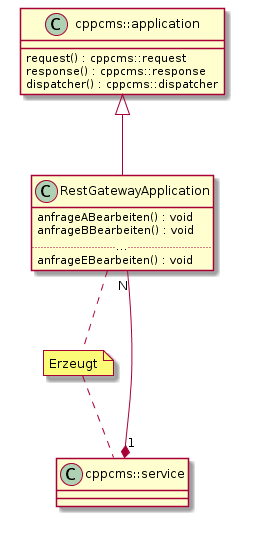
\includegraphics[scale=0.5]{praktikumsbericht.png}
\caption{CPPCMS Klassendiagramm}
\label{fig:cppcms_class_diagram}
\end{figure}

Ein Fehler der während der Anfrage gegenüber dem Marktrechner auftreten kann ist eine Zeitüberschreitung, falls dieses sich in einem bestimmten Zeitraum nicht mit einer Antwort zurückgemeldet hat. Als Antwort soll dem Client der HTTP-Statuscode 504 (Timeout) gesendet werden. Für alle anderen auftretenden Fehler soll der HTTP-Statuscode 500 (Internal server error), für interne Server Fehler, Nutzung finden.

Zum TCP-Verbindungsaufbau gegen das LAN-Gateway des Marktrechners werden Funktionen des Qt-Frameworks genutzt, um Telegramme zu senden und empfangen.

\begin{comment}
@startuml
class TcpClient {
	telegrammErzeugen(QByteArray) : QByteArray 
	telegrammSenden(QByteArray) : QByteArray 
}
@enduml
\end{comment}

\begin{figure}[h]
\centering
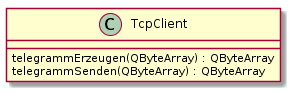
\includegraphics[scale=0.5]{praktikumsbericht_001.png}
\caption{CPPCMS Klassendiagramm}
\label{fig:cppcms_class_diagram}
\end{figure}

Die Klasse TcpClient soll über die Methode "telegrammErzeugen()", aus den Bytedaten, die die Methode für das Telegramm zusammengebaut hat, ein Telegramm schaffen, welches das LAN-Gateway versteht. Die Methode "telegrammSenden()" baut eine Verbindung zum Gateway auf, sendet das Telegramm und liefert die Daten der Antwort.

\subsubsection{Implementierung}

Der cppcms::service nutzt eine Event-Loop auf dem Haupt-Thread des Programmes. Wird er gestartet übernimmt er die Kontrolle der Ausführung. Die Auflistung \ref{lst:init_service} zeigt wie zunächst ein neues service-Objekt erzeugt wird. Der config-Parameter beinhaltet u. a. den Port auf dem gelauscht werden soll. In Zeile 2 wird über die Klasse RestGatewayApplication informiert, von welcher der service neue Objekte erzeugen kann. In Zeile 3 wird der service gestartet, wodurch er die erwähnte Kontrollübername durchführt.

\lstset{language=C++}
\begin{lstlisting}[caption=Service initialisieren, label=lst:init_service, frame=single, numbers=left, tabsize=3, captionpos=b]
cppcms::service service(config);
service.applications_pool().mount(
   cppcms::applications_factory<RestGatewayApplication>()
);
service.run();
\end{lstlisting}

Die RestGatewayApplication beinhaltet fünf Methoden zur Behandlung der fünf REST-Anfragen, welche für die erste Iteration ausgewählt wurden. Im Konstruktor muss die RestGatewayApplication anführen, für welche Anfrage der cppcms::service, welche Methode aufrufen soll. Dazu wird ein Regulärer Ausdruck gegen die URI der Anfrage abgeglichen. Im Fall eines Treffers wird die angegebene Methode aufgerufen, welche eine Antwort auf die Anfrage liefern soll. In der Auflistung \ref{lst:regex_dispatching} wird eine solche Zuweisung durchgeführt. Der erste Parameter ist der reguläre Ausdruck. Die in Klammern gekennzeichneten Teile eines Ausdrucks werden als Parameter an die zugewiesene Methode übergeben, welche im zweiten Parameter benannt wird. Über die Existenz eines Parameters im Regulären Ausdruck wird über einen Integer-Parameter hingewiesen. Zeile 5 und 6 zeigen zwei Integer-Parameter, mit den Werten eins und zwei. Diese Werte sind allerdings vollkommen belanglos, denn lediglich die Methodensignatur ist entscheidend für Gesamtanzahl an Parametern. Zur verbesserten Lesbarkeit können diese, wie in diesem Beispiel, durchnummeriert werden. Maximal vier Parameter werden dadurch von CPPCMS unterstützt.

\lstset{language=C++}
\begin{lstlisting}[caption=URI Zuweisung mit Regulärem Ausdruck, label=lst:regex_dispatching, frame=single, numbers=left, tabsize=3, captionpos=b]
dispatcher().assign(
	"REST/1.0/controller/(\\w+)/datapoint/(\\w+)", 
	&RestGatewayApplication::controller_dp,
	this,
	1,
	2
);
\end{lstlisting}

Parameter in der URI, wie sie beim HTTP-GET vorkommen können, werden von CPPCMS nicht in der Überprüfung des Regulären Ausdrucks berücksichtigt. Zugriff auf diese erlangt die behandelnde Methode über geerbte Methoden. Anhand ihres Namens sind diese abrufbar. In Auflistung \ref{lst:request_parameter} wird der "format"-Parameter ausgelesen. Weitere Parameter lassen sich analog auslesen.

\lstset{language=C++}
\begin{lstlisting}[caption=Anfrage-Parameter auslesen, label=lst:request_parameter, frame=single, numbers=left, tabsize=3, captionpos=b]
request().get("format");
\end{lstlisting}

Die für eine Anfrage aufgerufene Methode wird die für sich relevanten Parameter aus der HTTP-Anfrage auslesen. Anhand dieser wird dann ein parametrisierter Nutzdatenteil für ein Telegramm erstellt. Mit dem TcpClient kann dieses Telegramm erzeugt und gesendet werden. Details hierzu unterliegen dem Firmengeheimnis und können nicht angeführt werden.

Das als Antwort erhaltene Telegramm muss von der Methode interpretiert werden, damit anschließend ein Antwortdokument erzeugt werden kann. Zum Bauen dieses Dokumentes in XML wird das in Auflistung \ref{lst:qt_dom} gezeigt Qt XML-Module genutzt. Der Fall JSON wird in Auflistung \ref{lst:cppcms_json} mit dem cppcms::json-Modul gezeigt. Beide Dokumente beinhalten eine Versionnummer, den Zeitstempel der Erzeugung und einen interpretieren Inhalt. Beides sind abstrakte Beispiele, zur Demonstration der Module-APIs.

\lstset{language=C++}
\begin{lstlisting}[caption=Antwortdokument bauen mit Qt-XML, label=lst:qt_dom, frame=single, numbers=left, tabsize=3, captionpos=b]
QDomDocument antwort;
QDomElement antwortTag = antwort.createElement("antwort");
antwortTag.setAttribute("version", "1.0");
antwortTag.setAttribute("zeitstempel", aktuelleZeitUTC());
QDomText antwortInhalt = {...}
antwortTag.appendChild(antwortInhalt);
antwort.appendChild(antwortTag);
\end{lstlisting}

\lstset{language=C++}
\begin{lstlisting}[caption=Antwortdokument bauen mit CPPCMS-JSON, label=lst:cppcms_json, frame=single, numbers=left, tabsize=3, captionpos=b]
cppcms::json antwort;
antwort["version"] = "1.0";
antwort["zeitstempel"] = aktuelleZeitUTC();
antwort["inhalt"] = {...}
\end{lstlisting}

Das fertige Dokument wird als String der Antwortroutine von CPPCMS übergeben. In Auflistung \ref{lst:response} wird zunächst der Typ des Dokumentes, sowie die Schriftzeichenkodierung gesetzt. Dann wird das Dokument als String übergeben.

\lstset{language=C++}
\begin{lstlisting}[caption=Antwortdokument schreiben, label=lst:response, frame=single, numbers=left, tabsize=3, captionpos=b]
response().content_type("application/xml");
response().content_encoding("utf-8");
response().out() << antwort.toString();
\end{lstlisting}

\subsection{Zweite Iteration}

\subsubsection{Feinkonzept}

In der zweiten Iteration kam die Anforderung der Wartbarkeit von XML- und JSON-Rückgabedokumente hinzu. Der Zusammenbau der Dokumente in den Auflistungen \ref{lst:qt_dom} und \ref{lst:cppcms_json} ist zwar relativ kurz, dennoch ist der Quellcode weder besonders leicht zu lesen, noch wird bei seiner Betrachtung das endgültige Dokument sofort klar. Um zukünftig flexible Anpassungen an Kundenwünsche vornehmen zu können, soll eine Template-Engine eingesetzt werden. Diese soll es ermöglichen Templates zu erstellen, welche in externen Dateien gepflegt werden. Die Templates beinhalten die Struktur des Dokumentes und nutzen Platzhaltern für die eigentlichen Daten.

Die Auswahl an Templating-Engines scheint auf den ersten Blick überwältigend. Es gibt über ein Dutzend verschiedene, wovon die Meisten sich allerdings darauf spezialisiert haben, JSON Inhalte über Javascript in Templates mit eigener Syntax einzusetzen. Die mustache-Engine von Twitter ist eine der wenigen mit einer C++ Implementierung. Zudem wird sie als einzige regelmäßig gewartet. Neben einer klassischen C++ Implementierung, gibt es auch eine in Qt. Mustache unterstützt folgende, für die Implementierung wichtige, Platzhaltertypen. 

Einfache Platzhalter werden in mustache, Auflistung \ref{lst:placeholder}, durch einen Platzhalternamen zwei öffnende und zwei schließende geschweifte Klammern deklariert.

\begin{lstlisting}[caption=Einfache Platzhalter, label=lst:placeholder, frame=single, numbers=left, tabsize=3, captionpos=b]
{{name}}
\end{lstlisting}

Eine Aufzählung, Auflistung \ref{lst:placeholder_list}, wird über einen Platzhalter mit Hashtag vor dem Namen geöffnet und durch einen Platzhalter mit einem Slash vor dem Namen beendet.

\begin{lstlisting}[caption=Platzhalterliste, label=lst:placeholder_list, frame=single, numbers=left, tabsize=3, captionpos=b]
{{#liste}}
	{{item_name}}
{{/liste}}
\end{lstlisting}

\subsubsection{Implementierung}

Die Platzhalterersetzung finden in der Qt-Implementierung anhand von Hash-Schlüsseln statt. In der Auflistung \ref{lst:templateData} werden einem Hash über die Schlüssel "version" und "zeitstempel" die Werte "1.0" und der aktuelle Zeitstempel zugewiesen.

\lstset{language=C++}
\begin{lstlisting}[caption=Antwortdokument schreiben, label=lst:templateData, frame=single, numbers=left, tabsize=3, captionpos=b]
QVariantHash templateData;
templateData["version"] = "1.0";
templateData["zeitstempel"] = aktuelleZeitUTC();
\end{lstlisting}

Der Wert eines Schlüssels kann auch eine Liste sein. Die Liste muss aus einer Menge an Hashes bestehen. Auflistung \ref{lst:templateDataList} zeigt eine Liste mit Hashes, welche Informationen über mehrere Zähler beinhalten.

\lstset{language=C++}
\begin{lstlisting}[caption=Antwortdokument schreiben, label=lst:templateDataList, frame=single, numbers=left, tabsize=3, captionpos=b]
QVariantList zaehlerListe;
for (int i = 0; i < anzahl_zaehler; i++) {
    QVariantHash zaehler_wert;
    zaehler_wert["adresse"] = zaehler.adresse[i];
    zaehler_wert["prioritaet"] = zaehler.prioritaet[i];
    zaehlerListe << zaehler_wert;
}
templateData["zeahler_liste"] = zaehlerListe;
\end{lstlisting}

Das zugehörige Template für ein JSON-Dokument könnte wie in Auflistung \ref{lst:template} aussehen.

\lstset{language=json}
\begin{lstlisting}[caption=Antwortdokument schreiben, label=lst:template, frame=single, numbers=left, tabsize=3, captionpos=b]
{
	"Version" : "{{version}}",
	"Zeitstempel" : "{{zeitstempel}}",
	"Zaehler" : [ 
		{{#zaehler_liste}} 
			{ 
				"Adresse" : {{adresse}},
				"Prioritaet" :  {{prioritaet}}
			},
		{{/zaehler_liste}}
	]
}
\end{lstlisting}

Die Methode, welche eine Anfrage bearbeitet, erzeugt aus der interpretierten Antwort die Hashes. Die Flexibilität von Templates zeigt sich dadurch, dass Änderungen, ohne erneutes kompilieren und starten des Programms, vorgenommen werden können. Hierzu müssen lediglich die Templatedateien ausgetauscht werden.

\subsection{Dritte Iteration}

\subsubsection{Feinkonzept}

Die Architektur der ersten Iteration \ref{sec:it_1} ermöglicht es, beliebig viele, gleichzeitige Anfragen, an einen Marktrechner, zu stellen. Dessen Gateway akzeptiert jedoch nur eine limitierte Anzahl an Verbindungen. Um dem gerecht zu werden, müssen die folgende Anforderungen erfüllen werden. Erstens, unter allen Anfragen darf es nur eine Verbindung zwischen dem RestGateway und einem Marktrechner geben. Gleichzeitig dürfen beliebig viele, verschiedene Marktrechner, zur selben Zeit, angefragt werden (1:N). Zweitens, Anfragen die aufgrund der Verbindungsrestriktion nicht direkt verarbeitet werden können, müssen nach dem First-in, First-out Verfahren abgearbeitet werden. Drittens, Anfragen die länger benötigen als der Standard HTTP-Timeout, von 30 Sekunden, müssen mit dem HTTP Statuscode 202 und einer URI, für Clientseitiges polling, quittiert werden. Der Client muss diese URI solange Anfragen bis seine Antwort vorliegt. Viertens, liegt nach 3 Minuten keine Antwort des Marktrechners vor wird die Anfrage mit dem HTTP-Statuscode 504 verworfen. Fünftens, alle anderen Fehler sollen mit HTTP-Statuscode 500 an den Client gemeldet werden. In der Abbildung \ref{fig:request_state} sind die folgenden Anforderungen als Zustände einer Anfrage zu sehen.

\begin{comment}
@startuml
note left of Neu 
	Telegramm wurde gebaut
	und	soll an den Marktrechner
	gesendet werden. 
end note	
[*] --> Neu
Neu --> Bearbeitung: [Markrechner frei]\nMarktrechner anfragen/\nAnfrage-Telegramm senden
Neu --> Warteschlange: [Markrechner belegt]\nwarten

Warteschlange --> Bearbeitung: [Markrechner frei]\nMarktrechner anfragen/\nAnfrage-Telegramm senden
Warteschlange--> Warteschlange: [Markrechner belegt]\nwarten

Bearbeitung --> [*]: [Anfragezeit < 30s]\nAntwort-Telegramm\nsenden
Bearbeitung --> Gespeichert: [Anfragezeit > 30s]\nAntwort-Telegramm\nspeichern
Bearbeitung --> Zeitüberschreitung: [Anfragezeit > 3min]\nBearbeitung abbrechen

note left of Gespeichert 
	Antwort wird auf
	Polling-Anfrage des
	Client gesendet.
end note	
Gespeichert -->[*]: Antwort-Telegramm\nsenden
note right of Zeitüberschreitung 
	Zeitüberschreitung wird
	auf Polling-Anfrage des
	Client gesendet.
end note	
Zeitüberschreitung -->[*]: Zeitüberschreitungs-\nmeldung senden

@enduml
\end{comment}

\begin{figure}[h]
\centering
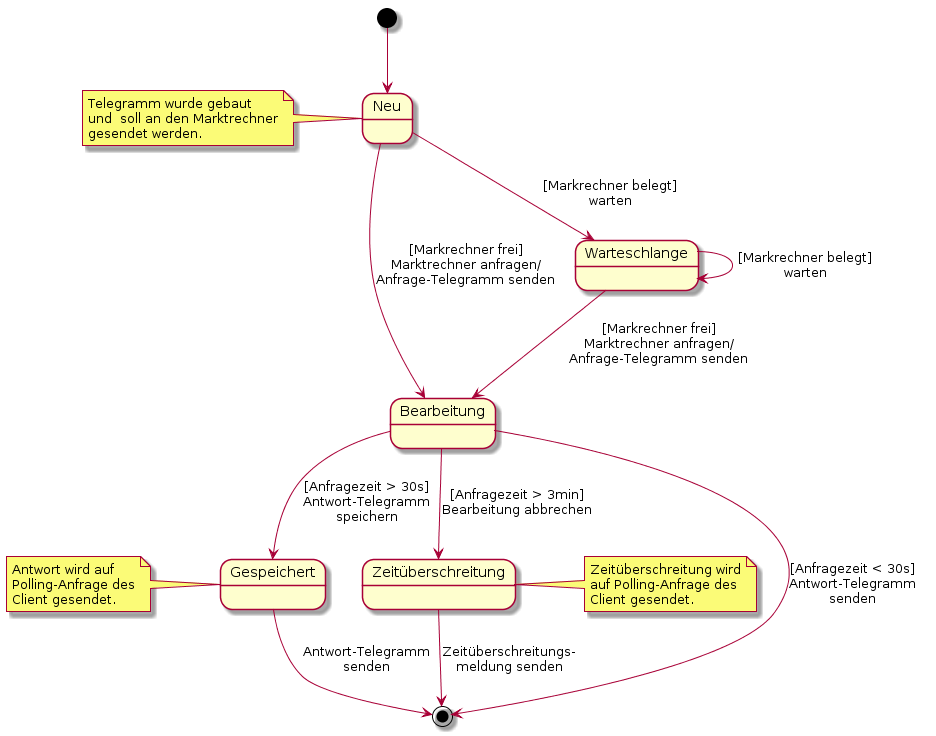
\includegraphics[scale=0.4]{praktikumsbericht_002.png}
\caption{Anfrage Zustandsdiagramm}
\label{fig:request_state}
\end{figure}

Der cppcms:service erzeugt eigenhändig neue Objekte von der Klasse RestGatewayApplication, wann immer eine neue Anfrage ankommt. Dadurch ist es nicht möglich zu kontrollieren, ob bereits eine Verbindung zu einem Marktrechner besteht. Aus diesem Grund wurde die Kontrollinstanz RequestManager eingeführt, welcher in einem zweiten Thread läuft. In Abbildung \ref{fig:architektur_requests} ist zu sehen, dass anstatt den Marktrechner direkt zu kontaktieren, delegiert die RestGatewayApplication diese Aufgabe an den RequestManager. Der RequestManager erzeugt für jede Anfrage einen RequestWorker in einem neuen Thread, der die Anfrage mit dem Marktrechner abarbeitet. Damit der RequestManager mit RestGatewayApplication und RequestWorker Informationen austauschen kann, benötigt es einen Kommunikationskanal. Dieser wird über ZeroMQ-Sockets hergestellt und benutzt das In-Process Protokoll (inproc). Dieses ermöglicht Nachrichten direkt über den Arbeitsspeicher auszutauschen. 

\begin{figure}[h]
\centering
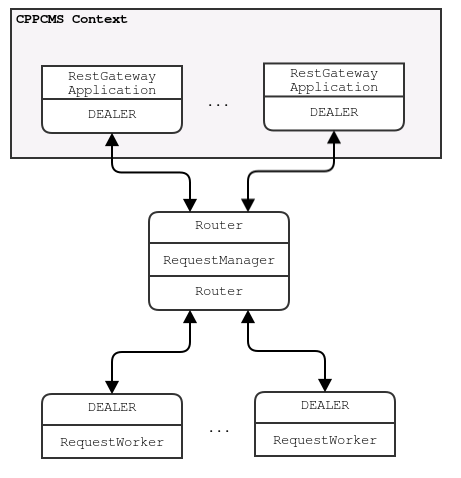
\includegraphics[scale=0.5]{Threads.png}
\caption{Multithreaded Architektur}
\label{fig:architektur_requests}
\end{figure}

Abbildung \ref{fig:architektur_requests} zeigt, dass der RequestManager zwei ROUTER-Sockets für n RestGatewayApplication DEALER-Sockets und m RequestWorker DEALER-Sockets hat. Der RequestManager bindet seine Sockets an die beiden inproc-Adresse "inproc://restgateway" und "inproc://worker". Dadurch kommt ein 1:N Verbindungsmuster zustande, im Vergleich TCP 1:1. Das reduziert die Anzahl der Sockets im RequestManager bei vielen Anfragen dramatisch. Damit eine Nachricht, welche an einen ROUTER gesendet wird, aber auch beim Empfänger ankommt, muss immer dessen Adresse angegeben werden. Diese sendet der DEALER automatisch in Form eines Universal Unique Identifier (UUID), beim Verbindungsaufbau. Ein Verbindungsaufbau muss immer von einem DEALER getätigt, da die UUID automatisch von ZeroMQ bei erzeugen des Sockets generiert wird.

Beim Austausch von Nachrichten zwischen verschiedenen Parteien ist es immer notwendig ein Protokoll zu erstellen. Dieses wurde in Angereicherte Backus-Naur-Form (ABNF) spezifiziert. Die Nachrichtentypen aus dem Protokoll werden in der Implementierung erläutert. Die Details der ABNF können hier nicht veröffentlicht werden.

\subsubsection{Implementierung}

Damit eine Anfrage asynchron verarbeitet werden kann wurden die folgende drei Nachrichten definiert. REQUEST sendet das gebaute Telegramm und etwaige Parameter der Anfrage. READY signalisiert, dass ein RequestWorker bereit ist eine Anfrage zu bearbeiten. Und RESPONSE sendet ein Telegramm, dass als Antwort vom Marktrechner empfangen wurde.

In Abbildung \ref{fig:async_request_handling} ist der Ablauf einer Anfrage durch einen RestClient, z.B. Browser, und anschließender asynchronen Verarbeitung dargestellt.

\begin{comment}
@startuml
autonumber
RestClient -> "cppcms::service": /REST/zaehler?\nformat=xml&\nip=10.0.25.10
activate "cppcms::service"

create RestGatewayApplication
"cppcms::service" -> RestGatewayApplication: new
"cppcms::service" ->> RestGatewayApplication: zaehler(xml)
activate RestGatewayApplication

RestGatewayApplication -> RestGatewayApplication: Telegramm\nbauen
RestGatewayApplication ->> RequestManager: <b>REQUEST</b>
activate RequestManager

create RequestWorker
RequestManager ->> RequestWorker: new
activate RequestWorker

RequestManager <<-- RequestWorker: <b>READY</b>
RequestManager ->> RequestWorker: <b>REQUEST</b>
RequestManager <<-- RequestWorker: <b>RESPONSE</b>
destroy RequestWorker

RestGatewayApplication <<-- RequestManager: <b>RESPONSE</b>
deactivate RequestManager

RestGatewayApplication -> RestGatewayApplication: XML bauen
"cppcms::service" <<-- RestGatewayApplication: XML
destroy RestGatewayApplication

RestClient <-- "cppcms::service": XML
deactivate "cppcms::service"
@enduml
\end{comment}

\begin{figure}[h]
\centering
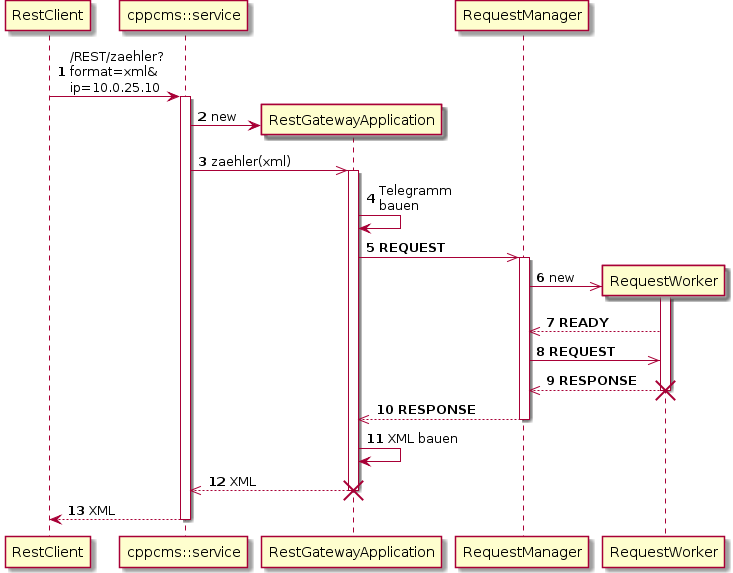
\includegraphics[scale=0.45]{praktikumsbericht_003.png}
\caption{Asynchrone Abarbeitung einer Anfrage}
\label{fig:async_request_handling}
\end{figure}

\begin{enumerate}[label=\protect\circled{\arabic*}]
\item Die Anfrage beginnt damit, dass ein RestClient eine HTTP Anfrage für eine Ressource stellt. In diesem Fall alle Zähler im XML-Format, vom Marktrechner mit der IP-Adresse 10.0.28.10. 
\item Der cppcms::service nimmt die Anfrage entgegen und erzeugt eine RestGatewayApplication. 
\item Anschließend wird die Methode zaehler(), der RestGatewayApplication, zur Anfragebearbeitung aufgerufen. 
\item Diese baut daraufhin das Telegramm, zur Anfrage aller Zähler.
\item Das Telegramm wird anschließend mit einer REQUEST-Nachricht an den RequestManager gesendet. 
\item Dieser erzeugt zur Bearbeitung einen RequestWorker. 
\item Der Worker meldet sich mit READY, nachdem er gestartet ist. 
\item Woraufhin er den REQUEST vom Manager weitergeleitet bekommt. 
\item Der RequestWorker baut eine Verbindung zum Marktrechner auf, stellt seine Anfrage, leitet die Antwort, in einer RESPONSE-Nachricht, an RequestManager zurück und beendet sich. 
\item Der RequestManager nimmt den RESPONSE und leitet ihn seinerseits an die RestGatewayApplication. 
\item Diese interpretiert die Antwort und baut das Antwortdokument in XML.
\item[\circled{12}\circled{13}] Das XML-Dokument wird dem cppcms::service übergeben, welcher es schlussendlich an den RestClient liefert.
\end{enumerate}

In den Anforderungen wird gefordert, die maximalen Anfragen, an einen Marktrechner, auf eine zu limitieren. Der RequestManager behält dazu die Kontrolle über Anfragen in Bearbeitung. In Abbildung \ref{fig:async_request_handling_multi_single} wird das Geschehen bei zwei gleichzeitig, an einen Marktrechner, gestellten Anfragen betrachtet. Um die Komplexität zu vereinfachen werden lediglich RequestManager und RequestWorker gezeigt. Alle ausgeblendeten Aufrufe funktionieren wie in Abbildung \ref{fig:async_request_handling}.

\begin{comment}
@startuml
autonumber
->> RequestManager: <b>REQUEST{1}</b>
activate RequestManager

create RequestWorker1
RequestManager ->> RequestWorker1: new
activate RequestWorker1

->> RequestManager: <b>REQUEST{2}</b>
RequestManager -> RequestManager: Warteschlange

RequestManager <<-- RequestWorker1: <b>READY{1}</b>
RequestManager ->> RequestWorker1: <b>REQUEST{1}</b>
RequestManager <<-- RequestWorker1: <b>RESPONSE{1}</b>
destroy RequestWorker1
<<-- RequestManager: <b>RESPONSE{1}</b>

create RequestWorker2
RequestManager ->> RequestWorker2: new
activate RequestWorker2

RequestManager <<-- RequestWorker2: <b>READY{2}</b>
RequestManager ->> RequestWorker2: <b>REQUEST{2}</b>
RequestManager <<-- RequestWorker2: <b>RESPONSE{2}</b>
destroy RequestWorker2
<<-- RequestManager: <b>RESPONSE{2}</b>

deactivate RequestManager
@enduml
\end{comment}

\begin{figure}[h]
\centering
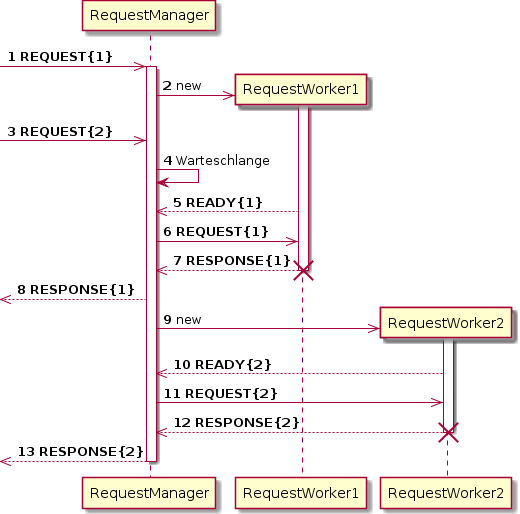
\includegraphics[scale=0.4]{praktikumsbericht_004.png}
\caption{Zwei Anfragen an einen Marktrechner}
\label{fig:async_request_handling_multi_single}
\end{figure}

\begin{enumerate}[label=\protect\circled{\arabic*}]
\item Für die erste eingehende Anfrage wird geprüft, ob bereits eine Verbindung zum angefragten Marktrechner besteht.
\item Da dies nicht der Fall ist wird ein neuer RequestWorker erzeugt. 
\item Die zweite eingehende Anfrage richtet sich an den selben Marktrechner. Die Prüfung ergibt, dass der angefragte Marktrechner bereits belegt ist.
\item Daher wird sie in eine Warteschlange eingefügt. 
\item Der zuvor erzeugte RequestWorker meldet sich mit READY.
\item Daraufhin bekommt er über REQUEST die Anfrage zugestellt. 
\item Sobald er eine Antwort vom Marktrechner erhält antwortet er mit RESPONSE. 
\item Der RESPONSE wird an den Aufrufer geleitet. Anschließend wird geprüft, ob weitere Anfragen für diesen Marktrechner vorliegen.
\item Da dies der Fall ist wird, für die Anfrage in der Warteschlange, eine neuer RequestWorker erzeugt. Die Schritte \circledsmall{10} - \circledsmall{13} sind dabei analog zu \circled{5} -  \circled{8}.
\end{enumerate}

Anfragen an unterschiedliche Marktrechner dürfen unabhängig voneinander gestellt werden. Abbildung \ref{fig:async_request_handling_multi_multi} zeigt diesen Fall.

\begin{comment}
@startuml
autonumber
->> RequestManager: <b>REQUEST{1}</b>
activate RequestManager
create RequestWorker1
RequestManager ->> RequestWorker1: new
activate RequestWorker1

->> RequestManager: <b>REQUEST{2}</b>
create RequestWorker2
RequestManager ->> RequestWorker2: new
activate RequestWorker2

RequestManager <<-- RequestWorker1: <b>READY{1}</b>
RequestManager ->> RequestWorker1: <b>REQUEST{1}</b>

RequestManager <<-- RequestWorker2: <b>READY{2}</b>
RequestManager ->> RequestWorker2: <b>REQUEST{2}</b>

RequestManager <<-- RequestWorker2: <b>RESPONSE{2}</b>
destroy RequestWorker2
<<-- RequestManager: <b>RESPONSE{2}</b>

RequestManager <<-- RequestWorker1: <b>RESPONSE{1}</b>
destroy RequestWorker1
<<-- RequestManager: <b>RESPONSE{1}</b>

deactivate RequestManager
@enduml
\end{comment}

\begin{figure}[h]
\centering
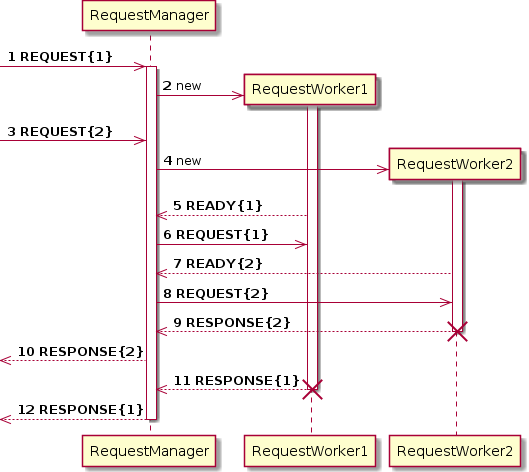
\includegraphics[scale=0.4]{praktikumsbericht_005.png}
\caption{Zwei Anfragen an unterschiedliche Marktrechner}
\label{fig:async_request_handling_multi_multi}
\end{figure}

\begin{enumerate}[label=\protect\circled{\arabic*}]
\item[\circled{1} \circled{3}] Für beide Anfrage wird geprüft, ob bereits eine Verbindung zum angefragten Marktrechner besteht.
\item[\circled{2} \circled{4}] Die Marktrechner für beide Anfragen sind nicht belegt. Deshalb wird jeweils ein ReuqestWorker erzeugt.
\item[\circled{5} - \circledsmall{12}] Die Bearbeitung der Anfragen läuft wie in den bereits erläuterten Abbildungen ab. Da beide Worker in eigenen Threads laufen ist es möglich, dass eine schnelle Anfrage eine langsame Anfrage überholt.
\end{enumerate}
In den drei vorgestellten Szenarien genügen drei Nachrichten des Protokolls, schließt man die Fehlerbehandlung zunächst einmal aus. Eine weitere Anforderung besagt jedoch, Anfragen die länger als der Standard HTTP-Timeout von 30 Sekunden laufen, müssen mit dem HTTP Code 202 und einer URI quittiert werden. An dieser URI kann der Client dann periodisch nach seiner Antwort oder dem Fortschritt fragen. Über die WAIT-Nachricht wird signalisiert, dass der HTTP-Timeout abgelaufen ist und mit der POLL-Nachricht, lässt sich die Antwort oder der Fortschritt erfragen. Mit den insgesamt fünf Nachrichten lässt sich das Polling wie in Abbildung \ref{fig:async_long_request_handling} realisieren.

\begin{comment}
@startuml
autonumber
RestClient -> "cppcms::service": /REST/zaehler?\nformat=xml&\nip=10.0.25.10
activate "cppcms::service"

create RestGatewayApplication
"cppcms::service" -> RestGatewayApplication: new
"cppcms::service" ->> RestGatewayApplication: zaehler(xml)
activate RestGatewayApplication

RestGatewayApplication -> RestGatewayApplication: Telegramm\nbauen
RestGatewayApplication ->> RequestManager: <b>REQUEST{123}</b>
activate RequestManager

create RequestWorker
RequestManager ->> RequestWorker: new
activate RequestWorker

RequestManager <<-- RequestWorker: <b>READY{123}</b>
RequestManager ->> RequestWorker: <b>REQUEST{123}</b>
...30 Sekunden später...
RestGatewayApplication <<-- RequestManager: <b>WAIT{123}</b>
RestGatewayApplication -> RestGatewayApplication: Generieren \neiner URI
"cppcms::service" <<-- RestGatewayApplication: HTTP 202 + URI
destroy RestGatewayApplication
RestClient <-- "cppcms::service": HTTP 202 + URI


RequestManager <<-- RequestWorker: <b>RESPONSE{123}</b>
destroy RequestWorker
RequestManager -> RequestManager: Antwort für \n123 speichern

RestClient -> "cppcms::service": /REST/1.0/poll/123
deactivate RequestManager

create RestGatewayApplication
"cppcms::service" -> RestGatewayApplication: new
"cppcms::service" ->> RestGatewayApplication: poll(123)
activate RestGatewayApplication

RestGatewayApplication ->> RequestManager: <b>POLL{123}</b>
activate RequestManager

RestGatewayApplication <<-- RequestManager: <b>RESPONSE{123}</b>
deactivate RequestManager

RestGatewayApplication -> RestGatewayApplication: XML bauen
"cppcms::service" <<-- RestGatewayApplication: XML
destroy RestGatewayApplication

RestClient <-- "cppcms::service": XML
deactivate "cppcms::service"
@enduml
\end{comment}

\begin{figure}[h]
\centering
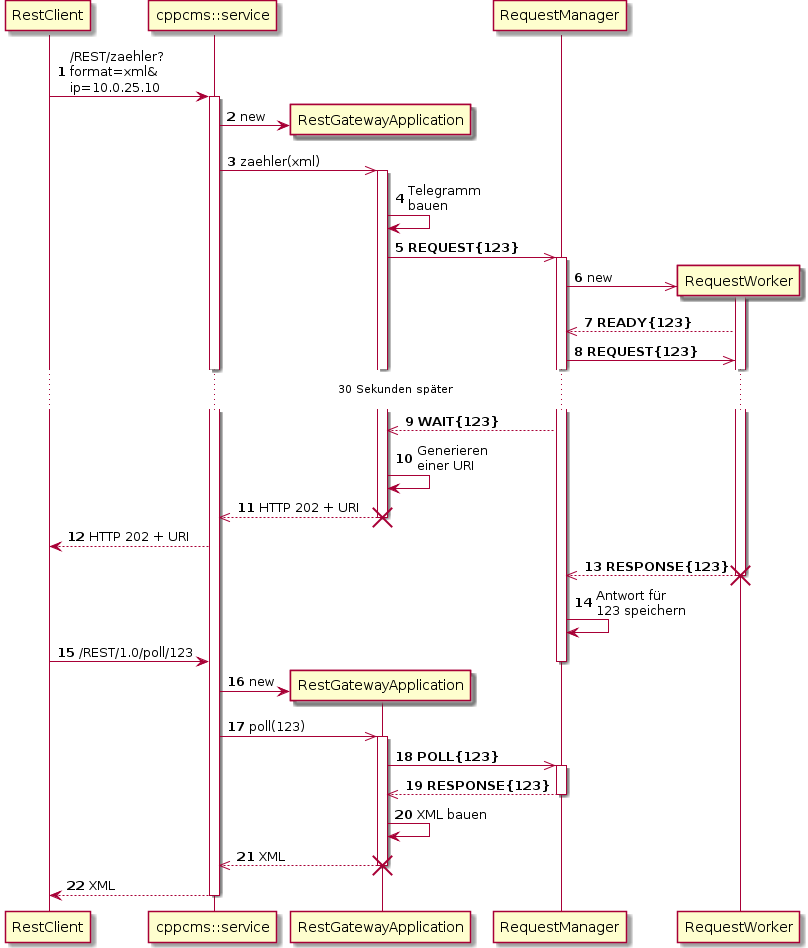
\includegraphics[scale=0.35]{praktikumsbericht_006.png}
\caption{Anfrage mit langer Bearbeitungszeit}
\label{fig:async_long_request_handling}
\end{figure}

Die Schritte \circledsmall{1} - \circledsmall{8} laufen wie gewohnt.
\begin{enumerate}[label=\protect\circled{\arabic*}]
\setcounter{enumi}{8}
\item Da innerhalb von 30 Sekunden keine Antwort des RequestWorkers vorliegt, sendet der RequestManager eine WAIT-Nachricht. 
\item Dadurch wird die RestGatewayApplication dazu veranlasst aus der Anfrage-ID, hier 123, eine URI zu generieren. 
\item[\circledsmall{11}\circledsmall{12}] Diese wird der Antwort angefügt und mit dem HTTP Statuscode 202 an den RestClient geliefert. 
\setcounter{enumi}{12}
\item Nach einer Zeit X sendet der RequestWorker die nun erhaltene Antwort. 
\item Der RequestManager nimmt diese an und speichert sie für den RestClient ab. 
\item Der RestClient pollt nach einer Zeit Y > X, für seine zuvor gestellte Anfrage. 
\item[\circledsmall{16}\circledsmall{17}\circledsmall{18}] Die daraufhin erzeugte RestGatewayApplication sendet daraufhin eine POLL-Nachricht an den RequestManager. 
\setcounter{enumi}{18}
\item Der nimmt die gespeicherte Antwort und sendet sie der RestGatewayApplication. 
\item[\circledsmall{20}\circledsmall{21}\circledsmall{22}] Mit der Antwort wird, das in der Anfrage geforderte XML-Dokument, gebaut und dem RestClient übermittelt.
\end{enumerate}

Sollte noch keine Antwort vorliegen, wenn der RestClient das Polling startet, wird der RequestManager erneut mit WAIT antworten. Liegt auch nach 3 Minuten keine Antwort vor, gibt es eine TIMEOUT-Nachricht vom RequestManager, welche die RestGatewayApplication mit dem HTTP Statuscode 504 an den RestClient weitergibt. Ist die beim Polling gesendete ID für eine Anfrage ungültig, z. B. wurde bereits abgeholt, schickt der RequestManager eine NO\_JOB-Nachricht. Diese wird von der RestGatewayApplication per HTTP Statuscode 400 an den RestClient quittiert. Sollte während der Bearbeitung ein Fehler auftreten, sendet der RequestManager eine ERROR-Nachricht, welche der RestGatewayManager mit HTTP-Statuscode 500 weiterleitet.

Somit besteht das vollständige Protokoll aus insgesamt 9 unterschiedlichen Nachrichten die zwischen RestGatewayApplication, RequestManager und RequestWorker hin und her gesendet werden.

\clearpage

\section{Wochenberichte}

\subsection{Woche 1 - W14 (01.04.14 - 04.04.14)}

Die erste Woche war geprägt von Einweisung, Einarbeitung und diversen Hilfsaufgaben. Am ersten Tag fand eine kurze Vorstellrunde mit dem Entwicklerteam statt. Im Anschluss ging es zum Arbeitsplatz, welcher sich aufgrund von Platzmangel, in einem anderen Büro befand. Die dort zur Verfügung gestellte Hardware war ein Desktop-PC mit Windows 7 Betriebssystem und ein Notebook mit Xubuntu 13.10 Betriebssystem. Zur Entwicklung wurde das Linux-Notebook verwendet. Der Desktop-PC diente hauptsächlich zur Anbindung an das Mail-System der Firma. Dort wurden Programme, Netzlaufwerke, Mail-System, Wiki und Issue-Tracking-System auf beide Systeme eingerichtet und erklärt. Die erste Praktikumsaufgabe war es, diverse CAN-Kabel zu bauen. Diese wurden benötigt, um Verbundsteuerungen, Kühlerregler und Marktrechner, eines neuen Teststandes, untereinander zu verbinden. Eine weitere Aufgabe in dieser Woche war es, einen UMTS-Stick unter Linux zu konfigurieren und die einzelnen Schritte in der Wiki-Software Confluence zu dokumentieren. Dieser soll einer Direktverbindung mit einem Kundensystem zu Wartungszwecken dienen. In der restlichen Zeit fand eine Einarbeitung zum Thema Sicherheit mit Bezug auf den lighttpd Webserver statt.

\subsection{Woche 2 - W15 (07.04.14 - 11.04.14)}

In der zweiten Woche wurde die Praktikumsaufgabe in Form eines Projekt beschrieben. Hierbei sollen Klienten über eine REST-Schnittstelle Informationen aus dem E*LDS System erfragen können. Die detaillierte Beschreibung des Projektes findet sich im Kapitel Projektbericht.
Für die Praktikumsaufgabe ergaben sich mehrere Teilaufgaben. Zunächst wurde die Dokumentation des proprietären Nachrichtenprotokolls gelesen. Anschließend konnten die Kenntnisse daraus anhand zweier ausgewählter Nachrichten auf einem Test-System ausprobiert werden. Hierzu wurde ein Test-Tool verwendet, das eine Anfrage über TCP an ein Gateway am CAN-Bus sendet und eine Antwort empfängt. Nachdem das Nachrichtenkonzept verstanden war, musste ein Framework zur Verarbeitung der REST-Anfragen gefunden werden. Da die Hauptkompetenz der Entwickler in C++ liegt, wurde das C++ Web-Framework CPPCMS evaluiert. Im Rahmen der Evaluierung wurde ein einfaches Testprogramm geschrieben, welches eine beliebige Anfrage auf der REST-Schnittstelle mit einen "Hallo Welt"-JSON Dokument beantwortet. CPPCMS bietet selbst keine Sicherheitsmechanismen an. Aus diesem Grund wurde ein lighttpd Webserver mit https konfiguriert und alle REST-Anfragen mittels FastCGI an CPPCMS weitergeleitet. Als erste konkrete Anfrage wurde der Abruf aller Teilnehmer auf dem CAN-Bus implementiert. Um an diese Information zu gelangen, wurde ein TCP-Client, nach Vorbild des Test-Tools, geschrieben. Die interpretierte Antwort des Gateways wird je nach Anfrageparameter per XML oder JSON Dokument, an die REST-Schnittstelle, geliefert.

\subsection{Woche 3 - W16 (14.04.14 - 17.04.14)}

In der dritten Woche wurden weitere REST-Schnittstellen und proprietäre Nachrichten an das E*LDS System umgesetzt. Anhand der zweiten zu sendenden Nachricht wurde eine Regelmäßigkeit in der REST-Anfrage/-Antwort und E*LDS Anfrage/-Antwort entdeckt. Um Redundanzen für weitere Nachrichten zu vermindern, wurde der Aufbau von E*LDS Anfragen/-Antworten sowie der REST-Schnittstellen in einem XML-Dokument beschrieben. Anschließend wurde ein Skript in GSL (https://github.com/imatix/gsl) geschrieben. GSL ist ein Universeller Code Generator, welcher es ermöglicht, aus XML-Daten Programmcode zu generieren. Der generierte Programmcode besteht aus dem REST-Endpunkt für die REST-Anfrage, der E*LDS-Anfrage, der Interpretation der E*LDS Antwort, sowie der Ausgabe als XML- oder JSON-Dokument. Um beim Testen Änderungen am Testsystem vorzunehmen, ohne Probleme für andere Entwickler zu verursachen, wurde ein CI4000 Marktrechner mit integriertem Lan-Gateway aufgesetzt. Das Software-Image auf Basis eines Embedded-Linux wird über eine serielle Leitung eingespielt. Sobald eine IP-Adresse gesetzt ist, kann man sich per ssh auf den Marktrechner verbinden, um Services zu starten oder weitere Konfigurationen vorzunehmen.

\subsection{Woche 4 - W17 (22.04.14 - 25.04.14)}

In der vierten Woche waren Templatessprachen und eine neuer Arbeitsplatz Hauptaugenmerk. Nach Implementierung einer komplexeren Anfrage und Antwort aus dem E*LDS System stellte sich heraus, dass das generieren von XML oder JSON, anhand des Aufbaus der E*LDS Antwort, Einzellösungen im XML und im Skript verursacht. Um die flache Struktur der E*LDS-Antworten in logisch geordnete XML- und JSON-Dokumente zu überführen wurde entschieden Templates zu verwenden. Die meisten Template-Engines nehmen Daten im JSON-Format und setzen diese per JavaScript in ein Template ein. Die Template-Engine mustache von Twitter überzeugte durch eine einfache Templatessprache und eine Implementierung in C++/QT. Diese machte es sehr einfach, Daten in Hashes zu referenzieren. Dazu wurde das Skript angepasst, sodass interpretierte E*LDS-Antworten automatisch in Hashes überführt werden. Weiterhin wurde der Programmcode in dieser Woche einem Subversion Versionskontrollsystem hinzugefügt. Dafür wurde das Projekt an die Strukturen anderer Projekte angepasst und eine Readme-Datei zur Erklärung des Skriptes angelegt. Am Ende der Woche musste dann ein neuer Arbeitsplatz bezogen werden, da der Alte für einen neuen Mitarbeiter benutzt werden würde. Mit dem Umzug in das Büro des Praktikumsbetreuers musste die bisherige Hardware gegen und ein Notebook mit Windows 7 Betriebssystem und einer Ubuntu Virtual-Maschine getauscht werden. Um die Arbeit an dem Projekt fortsetzen zu können, wurde der Freitag genutzt, um die bisherige Toolchain auf dem neuen Notebook zu installieren und zu konfigurieren.

\subsection{Woche 5 - W18 (28.04.14 - 02.05.14)}

In der fünften Woche wurden Templates flächendeckend eingeführt und Programmcode aufgeräumt. Zunächst wurden für alle REST-Antworten mustache Templates erstellt. Durch deren Benutzung konnte unnötiger Skriptcode entfernt werden, welcher in erster Iteration CPPCMS-JSON und Qt-XML generiert hatte. Zudem konnten einige XML-Attribute, die spezifisch für diese Generierung angelegt worden waren, entfernt werden. Im XML wird lediglich ein Verweis auf das XML- oder JSON-Template erstellt. Insgesamt wurde dadurch ca. 1/4 an Programmcode gespart. In einer Kontrolle der XML und JSON Antworten wurde festgelegt, dass jedes Dokument einen Zeitstempel seiner Erstellung und eine Versionsnummer tragen soll. Die Zeitstempel werden als UNIX Zeitstempel in Sekunden seit 1970 erzeugt. Die Zeitzone wurde auf UTC+0 festgelegt. Eine Nebenaufgabe in dieser Woche war die Erörterung der Migrationsfähigkeit von Wiki-Inhalten der alten Wiki Software, Tiki-Wiki, nach Confluence. Der letzte Tag der Woche wurde genutzt, um die Wochenberichte der bisherigen Wochen zu schreiben.

\subsection{Woche 6 - W19 (05.05.14 - 09.05.14)}

In der sechsten Wochen wurde die Projektdokumention auf einen aktuellen Stand gebracht und eine Aufgabenverwaltung eingesetzt. Zum Start der Woche wurden alle implementierten Schnittstellen im Detail mit Eingabe- und Ausgabebeispielen beschrieben. Des Weiteren wurden die REST-URIs, welche zu dem Zeitpunkt einem Mix an deutscher und englische Sprache bestanden, einheitlich ins englische übersetzt. Durch die Übersetzung mussten die XML-Beschreibungen angepasst und der Programmcode neu generiert werden. Anschließend wurden das weitere Vorgehen im Projekt und neue Aufgaben besprochen. Die besprochenen Aufgaben wurden dann in das Projektverfolgungstool Jira eingepflegt, um einen besseren Überblick zu behalten. Insgesamt wurden weitere vier Schnittstellen in dieser Woche implementiert, darunter der Abruf von Istwert-Informationen. Dieser Abruf ist historisch gewachsen und bedurfte einer längeren Einarbeitung. Diese Informationen wurden in dieser Woche auch von einem anderen Mitarbeiter benötigt, worauf das erst kürzlich angeeignete Wissen über diese Schnittstelle weitergegeben werden konnte. 

\subsection{Woche 7 - W20 (12.05.14 - 16.05.14)}

In der siebten Woche wurde ein Konzept zur asynchronen Verarbeitung von REST-Anfragen entwickelt und ein "Proof of Concept" implementiert. Um zukünftig alle E*LDS Nachrichten über die REST-Schnittstelle abwickeln zu können, wurde eine generische Schnittstelle implementiert. Diese erhält Anfragen über HTTP-POST. Diese Anfragen enthalten eine bereits fertige, im E*LDS Protocol kodierte Nachricht, welche direkt an das Gateway weitergereicht werden kann. Die Antwort wird unverändert, ohne Interpretation, an den Aufrufer gesendet. Damit es nicht zu Problemen bei der Bytedarstellung kommt, wird der Payload auf beiden Wegen per BASE64 kodiert.

Bisher war es möglich, beliebig viele Anfragen auf einmal zu senden, die alle simultan bearbeitet wurden. Da jeweils nur eine Verbindung zu einem Marktrechner sinnvoll ist, konnte man dadurch leicht das Programm zum Absturz bringen. Zudem wurde der HTTP-Standard-Timeout von 30 Sekunden bei einigen Anfragen überschritten, was zu Problemen beim Aufrufer führte. Vor diesem Hintergrund wurde ein Konzept zur asynchronen Verarbeitung entwickelt. Hierbei darf max. eine Anfrage pro E*LDS System gleichzeitig gestellt werden. Weitere Anfragen werden aufgereiht und nach First-come, first-served (FCFS) abgearbeitet. Des Weiteren sollen Anfragen, welche länger als der HTTP-Timeout brauchen, mit einer URL zum Abholen der Antwort quittiert werden. Ist noch keine Antwort vorhanden, wenn ein Client die URL anfragt, wird er mit einer Wartemeldung vertröstet. Da die Verarbeitung in verschiedenen Threads abläuft, wurden drei Verfahren zum Datenaustausch getestet. Zunächst wurde ein Zeiger auf ein gemeinsames Objekt zwischen Threads geteilt. Da die Erzeugung des Threads zur Bearbeitung der REST-Anfrage allerdings unter der Kontrolle von CPPCMS liegt, war dies extrem umständlich und fehleranfällig. Als zweites wurde ein Stück gemeinsam genutzter Speicher (Shared Memory) benutzt. Da dieser mit einer festen Größe unterliegt, gab es hierbei jedoch Probleme bei einer bestimmten Menge von Anfragen. Danach wurde das Concurrency Framework ZeroMQ benutzt, um Nachrichten über die inproc-Schnittstelle zwischen den Threads hin und her zu schicken. Auf Basis dessen wurde eine äußert robuste und skalierbare asynchrone Verarbeitung geschaffen.

\subsection{Woche 8 - W21 (19.05.14 - 23.05.14)}

In der achten Woche wurde die asynchrone Abarbeitung von REST-Anfragen umgesetzt und die generische Schnittstelle angepasst. Die generische Schnittstelle erwartet den Payload BASE64 kodiert im HTTP POST Content. Dadurch entfällt jedoch die Möglichkeit, Parameter anzuhängen. Deshalb wurden die Anfrage und die Antwort in einen XML-Umschlag gewickelt. So ist es möglich weitere Parameter wie Marktrechner-IP oder Zeitstempel mitzugeben.

Die asynchrone Verarbeitung wurde in das Skript zur Generierung der REST-Schnittstellen eingepflegt. Dieses enthielt einen Großteil an Logik zur Behandlung von Spezialfällen. Um diese entfernen zu können, wurde eine Oberklasse für die REST-Schnittstellen erstellt, welche diese Spezialfälle behandelt. Zudem musste das Protokoll um Meta-Daten erweitert werden. Diese werden zum Erstellen des Rückgabedokumentes benötigt. Notwendig ist dieser Mechanismus geworden, weil beim Polling Anfrage und Antwort in unterschiedlichen REST-Anfragen gesendet werden und es keinen gemeinsamen Kontext zwischen den Anfragen gibt.

Diese Woche gab es auch erneut eine Nebenaufgabe. Es wurde auf einen HP MicroServer, bestehend aus fünf Festplatten Steckplätzen, Ubuntu 12.04.4 aufgespielt. Anschließend wurde Software installiert, die benötigt wird, um die Softwareprojekte des Teams zu kompilieren. Die Hauptaufgabe des Server wird zukünftig die automatische Testausführung sein. Dazu wurde ein Jenkins Continuous Integration Server installiert. Dieser ermöglicht das automatische Abarbeiten von Aufgaben zu bestimmten Auslösern. Diese Auslöser können zeit- oder ereignisgesteuert sein. Die automatisierten Tests sollen später zeitgesteuerte, jede Nacht ausgeführt werden. Für die Wartung wurde abschließend ein SSH- und RDP-Server aufgesetzt.

\subsection{Woche 9 - W22 (26.05.14 - 30.05.14)}

In der neunten Woche wurden Lasttests geschrieben und das Logging auf dem Testserver vereinheitlicht. Die asynchrone Abarbeitung hat beim Entwickeln gegen einzelne sporadisch ankommende REST-Anfragen, welche über den Browser abgesetzt wurden, ohne Auftreten von Problemen funktioniert. Da dies im produktiven Einsatz jedoch nicht immer der Fall ist, wurden automatisierte Lasttests geschrieben, diese simulieren ein plötzliches Aufkommen vieler Anfragen. In diesem Zuge konnten drei große Bugs identifiziert und gelöst werden. Weiterhin wurde mit Hilfe eines anderen Entwicklers der Quellcode einem Review unterzogen. Anschließend wurden Teile vereinfacht und sicherer gemacht.

Die Nebenaufgabe der Woche war das Logging auf dem Testserver, über syslog, zu vereinheitlichen. Hierzu wurde der Server syslog-ng installiert. Anschließend wurden diverse Regeln und Filter konfiguriert, um die wichtigsten Log-Nachrichten, im selben Format, in eine Datei umzuleiten. Später soll ein Tool installiert werden, dass den Inhalt dieser Logdatei aufbereitet und über ein Web-Interface visualisiert.	

\subsection{Woche 10 - W23 (02.06.14 - 06.06.14)}

In der zehnten Woche wurde der Testserver an allen Fronten weiter konfiguriert. Der zuvor installierte Jenkins Server ist standardmäßig für das Testen von Java Applikationen ausgelegt. Deshalb mussten einige Plugins installiert werden, die Qt-Tests automatisch auszuführen, auszuwerten und zu visualisieren. Weitere Plugins machen die Benutzerverwaltung komfortabler. 

Des Weiteren wurde das Logging Web-Interface installiert. Während der Konfiguration stellte sich allerdings heraus, dass syslog-ng nicht ausreichend unterstützt wird.

Die in dieser Woche gelieferten Festplatten für den Testserver wurden eingebaut und im Software-RAID 1 konfiguriert. Als Dateisystem wird Ext4 verwendet.

\subsection{Woche 11 - W24 (09.06.14 - 13.06.14)}

In der elften Woche wurde das Web-Interface für syslog-ng erneut in Angriff genommen und weitere Aufgaben Jenkins zugewiesen. Das Web-Interface wurde durch ein Open-Source Tool umgesetzt. Durch einige kleiner Änderungen an der syslog-ng Konfiguration können nun die Logs im Browser angeschaut werden.
Damit der Jenkins Server seine Aufgaben auf dem Software-RAID 1 durchführen kann, wird dieses automatisch beim Systemstart gemountet. Um die Lasttests des RestGateways automatisch im nächtlichen Turnus auszuführen, wurden dieses mit Startparametern versehen, welche den Port festlegen. Diese Maßnahme war nötig, damit es nicht zum Konflikt mit anderen Services auf dem Testserver kommt. Um zukünftig auch auf einer Test-Hardware das nächtliche Image aufzuspielen und testen zu können, mussten zunächst die zuvor installierten Build-Tools konfiguriert werden. Das bauen des Images kann beschleunigt werden, wenn auf vor-kompilierte Module zugegriffen werden kann. Diese liegen auf einen NFS Laufwerk, welches automatisch während des Systemstart gemountet wird.
Des Weiteren wurde die RAID-Konfiguration durch eine Email Benachrichtigung erweitert, welche einen Mitarbeiter im Falle eines Festplattenausfall benachrichtigt. Zudem wurde versucht das RestGateway unter Windows zum Laufen zu bekommen. Dazu mussten die abhängigen Bibliotheken von CPPCMS und ZeroMQ mit MinGW kompiliert werden. Für CPPCMS mussten zunächst weiter fünf Abhängigkeit in Form von DLLs gefunden, heruntergeladen und zusammengepackt werden. Für ZeroMQ kann man sich bereits vorkompilierte  DLLs herunterladen. Die ZeroMQ Higher-Level Bindings für C (czmq), mussten allerdings kompiliert werden. Da hier auf dem aktuellen Master aufgesetzt wurde, mussten zunächst einige Patches getätigt und dem Projekt zurückgeführt werden, womit sich das Projekt kompilieren lies. Aufgrund fehlender MinGW und Windows Kenntnisse schlug das linken der DLL allerdings fehl, womit in dieser Woche keine lauffähige Version des RestGateway unter Windows zustande gebracht wurde.

\subsection{Woche 12 - W25 (16.06.14 - 20.06.14)}

In der zwölften und letzten Woche des Praktikums wurde XML diskutiert und überarbeitet. Die bisher in Templates erstellten XML-Dokumente wurden geprüft auf Konsistenz, Erzeugbarkeit, Weiterverarbeitung, Versionierbarkeit, Sinnhaftigkeit und Lesbarkeit. Unter Berücksichtigung dieser Aspekte wurden die XML-Templates zunächst vervollständigt und alle Tags und Attribute in Prosa übersetzt. Danach wurde der Aufbau von Listen und Elementen in eine einheitliche Struktur umgesetzt. Zum Schluss wurden zwei unterschiedliche Arten der Versionierbarkeit für eine größere Diskussionsrunde vorbereitet. Die restliche Zeit wurde genutzt, um den Praktikumsbericht inhaltlich zu vervollständigen.

\clearpage

\section{Fazit}

\subsection{Allgemeines Fazit}

Das Team Datentechnik, der Abteilung KGL, steht Innovationen sehr offen gegenüber. So wurden hier die eingesetzten Systeme Jira und Confluence erprobt, evaluiert und die Werteschöpfung, gegenüber den Altsystemen, für das gesamte Unternehmen herausgearbeitet. Das Team arbeitet mit einem agilen Vorgehen, welches Wurzeln in Scrum und Kanban hat. Entwickelt wird auf der Versionsverwaltung subversion. Arbeitsanweisungen werden mit dem Ticketing-System Jira, in den verschiedenen Workflowschritten Anforderungsanylyse, Implementierung und Testen, zwischen den Parteien kommuniziert. Wissen kann mit der Wiki-Software Confluence festgehalten und ausgetauscht werden.  Ein Jenkins Build-Server übernimmt zudem das nächtliche Bauen der Geräteimages und führt automatisiert Tests aus. Automation ist wichtig und deren Erweiterung war deshalb auch Teil der Praktikumsaufgaben. 

\subsection{Persönliches Fazit}

Die Wurzeln, der Firma Eckelmann, in der Hardwareentwicklung ist deutlich zu spüren. Zwar gehören schwergewichtige Entwicklungsmodelle im Team Datentechnik der Vergangenheit an, dennoch steht die moderne Softwareentwicklung noch am Anfang, mit jeder Menge Potential nach oben. Treibende Kraft hierbei ist Teamleiter Matthias Wolf, welcher durch seine Expertise für ein angenehmes Praktikumsumfeld und jede Menge neues Wissen gesorgt hat.

\clearpage
\section{Anhang}

Auf den folgenden Seiten sind die Stundennachweise zu finden.

\end{document}
